%%%%%%%%%%%%%%%%%%%%%%%%%%%%%%%%%%%%%%%%%
% Short Sectioned Assignment
% LaTeX Template
% Version 1.0 (5/5/12)
%
% This template has been downloaded from:
% http://www.LaTeXTemplates.com
%
% Original author:
% Frits Wenneker (http://www.howtotex.com)
%
% License:
% CC BY-NC-SA 3.0 (http://creativecommons.org/licenses/by-nc-sa/3.0/)
%
%%%%%%%%%%%%%%%%%%%%%%%%%%%%%%%%%%%%%%%%%

%----------------------------------------------------------------------------------------
%	PACKAGES AND OTHER DOCUMENT CONFIGURATIONS
%----------------------------------------------------------------------------------------

\documentclass[paper=a4, fontsize=11pt]{scrartcl} % A4 paper and 11pt font size

\usepackage[T1]{fontenc} % Use 8-bit encoding that has 256 glyphs
\usepackage{fourier} % Use the Adobe Utopia font for the document - comment this line to return to the LaTeX default
\usepackage[spanish]{babel} % English language/hyphenation
\selectlanguage{spanish}
\usepackage[utf8]{inputenc}
\usepackage{amsmath,amsfonts,amsthm} % Math packages
\usepackage{graphicx}

\usepackage{sectsty} % Allows customizing section commands
\allsectionsfont{\centering \normalfont\scshape} % Make all sections centered, the default font and small caps

\usepackage{fancyhdr} % Custom headers and footers
\pagestyle{fancyplain} % Makes all pages in the document conform to the custom headers and footers
\date{}
\fancyhead{} % No page header - if you want one, create it in the same way as the footers below
\fancyfoot[L]{} % Empty left footer
\fancyfoot[C]{} % Empty center footer
\fancyfoot[R]{\thepage} % Page numbering for right footer
\renewcommand{\headrulewidth}{0pt} % Remove header underlines
\renewcommand{\footrulewidth}{0pt} % Remove footer underlines
\setlength{\headheight}{5.6pt} % Customize the height of the header

\numberwithin{equation}{section} % Number equations within sections (i.e. 1.1, 1.2, 2.1, 2.2 instead of 1, 2, 3, 4)
\numberwithin{figure}{section} % Number figures within sections (i.e. 1.1, 1.2, 2.1, 2.2 instead of 1, 2, 3, 4)
\numberwithin{table}{section} % Number tables within sections (i.e. 1.1, 1.2, 2.1, 2.2 instead of 1, 2, 3, 4)

\setlength\parindent{0pt} % Removes all indentation from paragraphs - comment this line for an assignment with lots of text

%----------------------------------------------------------------------------------------
%	TITLE SECTION
%----------------------------------------------------------------------------------------

\newcommand{\horrule}[1]{\rule{\linewidth}{#1}} % Create horizontal rule command with 1 argument of height

\title{	
\normalfont \normalsize 
\textsc{UNIVERSIDAD DE CANTABRIA, DEPARTAMENTO DE FÍSICA MODERNA} \\ [20pt] % Your university, school and/or department name(s)
\horrule{0.5pt} \\[0.4cm] % Thin top horizontal rule
\huge Física de Partículas Elementales (G71) \\ % The assignment title
\normalsize 4 Curso - Grado de Física - Doble Grado Física Matemáticas - Ejercicios Tema 4
\horrule{2pt} \\[0.5cm] % Thick bottom horizontal rule
}

\begin{document}

\maketitle % Print the title

\vspace{-2.5cm}

%----------------------------------------------------------------------------------------
%	PROBLEM 1
%----------------------------------------------------------------------------------------
\textbf{Cuestión 1.} Calcular el branching ratio para el decaimiento $K^+\rightarrow\pi^+ + \pi^0$, teniendo en cuenta que la anchura parcial $\Lambda (K^+\rightarrow\pi^+ + \pi^0)=1.2\times 10^{-8}eV$ y 
la vida media del kaón $\tau(K^+)=1.2\times 10^{-8}s$.
\\
\\
%----------------------------------------------------------------------------------------
%       PROBLEM 2
%----------------------------------------------------------------------------------------
\textbf{Cuestión 2.} La sección eficaz de aniquiliación del proceso $e^+e^-\rightarrow\gamma\rightarrow\mu^+\mu^-$ viene dada por $\sigma =4\pi\alpha^2/3s$, donde $\alpha =1/137$. Calcula
la sección eficaz a $\sqrt{s}=50~GeV$, expresando la respuesta en unidades naturales (barns). Comparar el resultado con la sección eficaz total de colisión de protones a $\sqrt{s}=50~GeV$
que es aproximadamente 40~mb y comenta el resultado. 
\\
\\
%----------------------------------------------------------------------------------------
%       PROBLEM 3
%----------------------------------------------------------------------------------------
\textbf{Cuestión 3.} El flujo invariante Lorentz para el proceso $a + b\rightarrow 1 + 2$ en el sistema de centro de masas es $F=4p^*_i\sqrt{s}$ donde $p^*_i$ es el momento de las partículas
del estado inicial. Demostrar que la expresión correspondiente en el sistema en el que la partícula b está en reposo es:
\begin{equation*}
F=4m_bp_a
\end{equation*}
%----------------------------------------------------------------------------------------
%       PROBLEM 4
%----------------------------------------------------------------------------------------
\textbf{Cuestión 4.} Demostrar que el momento en el centro de masas de las partículas del estado inicial en un proceso de scattering con 2 partículas es:
\begin{equation*}
P_i^{*2}=\frac{1}{4s}[s - (m_1+m_2)^2][s - (m_1-m_2)^2]
\end{equation*}
%----------------------------------------------------------------------------------------
%       PROBLEM 5
%----------------------------------------------------------------------------------------
\textbf{Cuestión 5.} Dibuja el los dos diagramas de Feynman de más bajo orden para el scattering Compton $e\gamma\rightarrow e\gamma$.
\\
\\
%----------------------------------------------------------------------------------------
%       PROBLEM 6
%----------------------------------------------------------------------------------------
\textbf{Cuestión 5.} ¿Cuáles de los siguientes diagramas de Feynamn son válidos?
  
%\vspace{3cm}

\begin{figure}[!h]
\begin{center}
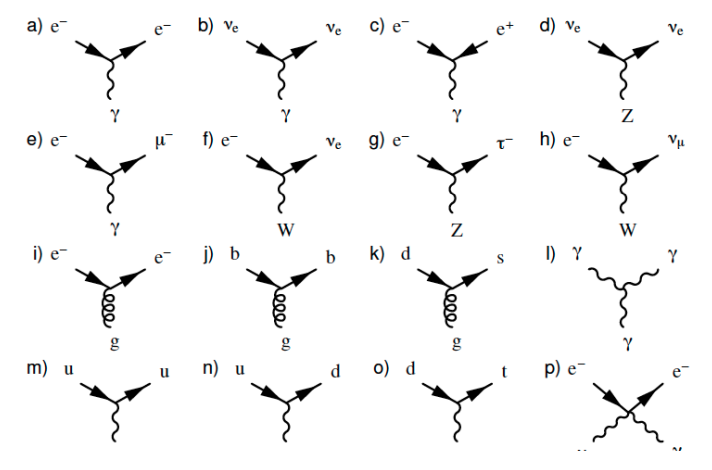
\includegraphics[width=0.6\linewidth]{feynman.png}
\end{center}
\end{figure}



\end{document}
